\documentclass[a4paper,fleqn,usenatbib]{mnras}
\pdfoutput=1
% MNRAS is set in Times font. If you don't have this installed (most LaTeX
% installations will be fine) or prefer the old Computer Modern fonts, comment
% out the following line
%\usepackage{newtxtext,newtxmath}
% Depending on your LaTeX fonts installation, you might get better results with one of these:
%\usepackage{mathptmx}
%\usepackage{txfonts}

% Use vector fonts, so it zooms properly in on-screen viewing software
% Don't change these lines unless you know what you are doing
\usepackage[T1]{fontenc}
\usepackage{ae,aecompl}
\usepackage{epstopdf}
\usepackage{aas_macros}
\usepackage{braket}
\usepackage{verbatim}
\usepackage{wrapfig}
\usepackage{booktabs}
\usepackage{amsfonts}
\usepackage{amsmath}
\usepackage{appendix}
\usepackage{graphicx}
\usepackage[usenames,dvipsnames]{color}
\usepackage[normalem]{ulem}
\usepackage{array}
\bibliographystyle{mnras}


\newcommand{\myemail}{samuelreay@gmail.com}
\newcommand{\tick}{\checkmark}
\newcommand{\gtick}{\color{ForestGreen} \tick }
\newcommand{\cross}{$\times$ }
\newcommand{\rcross}{\color{red} \cross }
\newcommand{\runz}{\textsc{Runz}}
\newcommand{\brac}[1]{\left( #1 \right)}
\newcommand*\mean[1]{\bar{#1}}
\newcommand\abs[1]{\left|#1\right|}
\newcommand {\etal} {\emph{~et~al.} }
\newcommand{\green}{\color{green}}
\newcommand{\blue}{\color{blue}}
\newcommand{\red}{\color{red}}
\newcommand{\orange}{\color{BurntOrange}}
\newcommand{\purple}{\color{Fuchsia}}
\newcommand{\hMpc}{h^{-1} {\rm Mpc}} % to be used in math mode
\newcommand{\camb}{\textsc{camb}}
\newcommand{\cosmomc}{\textsc{cosmomc}}

\newcommand{\kmsmpc}{km\,s$^{-1}$\,Mpc$^{-1}$}

\newcommand{\halofit}{\textsc{halofit}}
\newcommand{\specialcell}[2][c]{\begin{tabular}[#1]{@{}c@{}}#2\end{tabular}}



%\shortauthors{}
\title[MC Corrections for Bayesian Methods]{Monte Carlo Corrections for Bayesian Methods}

\author[S. R. Hinton et al.]{Samuel R. Hinton,$^{1,2}$\thanks{E-mail: \href{samuelreay@gmail.com}}
\\
% List of institutions
$^{1}$School of Mathematics and Physics, The University of Queensland, Brisbane, QLD 4072, Australia\\
$^{2}$ARC Centre of Excellence for All-sky Astrophysics (CAASTRO)
}
% These dates will be filled out by the publisher
\date{Accepted XXX. Received YYY; in original form ZZZ}

% Enter the current year, for the copyright statements etc.
\pubyear{2017}

\begin{document}


\label{firstpage}
\pagerange{\pageref{firstpage}--\pageref{lastpage}}
\maketitle



\begin{abstract}
I present a rigorous treatment for truncated or biased datasets by combining Bayesian analysis methods with Monte Carlo simulations.
\end{abstract}


%\vspace{35mm}

\section{Introduction}

Find some treatment of biased or truncated data before. Maybe \citet{Gull1989bayesian}.

\section{The perfect world}

In a perfect world, data is neither biased nor truncated. The data is perfect. Uncertainties are well quantified and normally distributed around true values. Presumably everything is also spherical and in a vacuum. Let us create a mock model in this perfect world. Let us observe a series of iid events $\vec{x}$, which is known perfectly and drawn from a normal distribution such that 
\begin{align}
\vec{x} \sim \mathcal{N}(\mu,\sigma)
\end{align}
If, having collected our observations of $\vec{x}$, we wanted to constrain $\mu$ and $\sigma$, this would be a simple task of modelling the posterior surface. Taking uniform priors on both parameters we simply wish to map the surface
\begin{align}
P(\mu,\sigma| \vec{x}) &\propto P(\vec{x} | \mu, \sigma) P(\mu, \sigma) \\
P(\mu,\sigma| \vec{x}) &\propto \prod_{i=1}^N \mathcal{N}(x_i | \mu, \sigma).
\end{align}
Generating a hundred data points with $\mu=100,\ \sigma=10$, we can recover our input parameters easily, as shown in Figure \ref{fig:perfect}.
\begin{figure}
	\begin{center}
		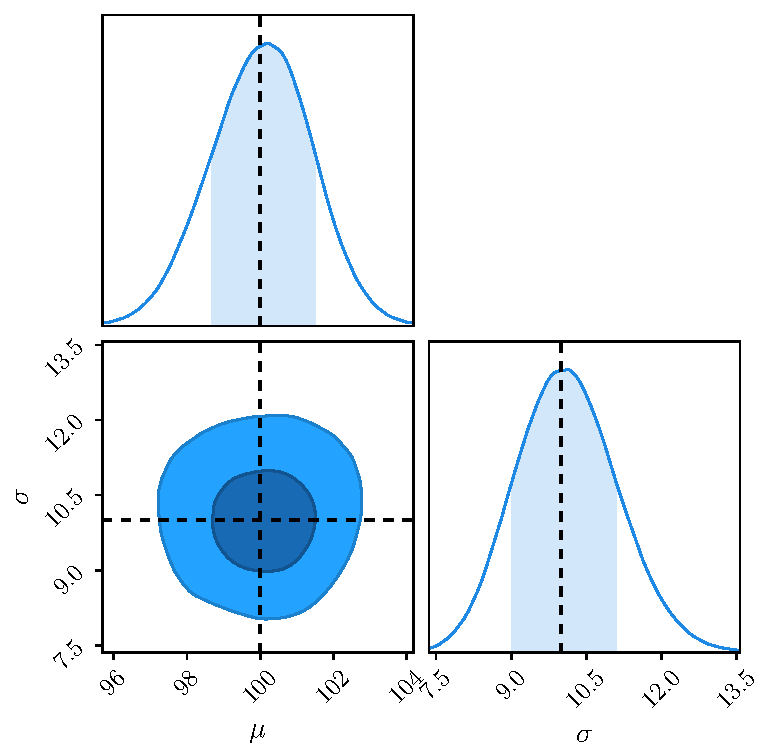
\includegraphics[width=\columnwidth]{example/perfect.pdf}
	\end{center}
	\caption{A systematic test of our perfect model, done by stacking the output chains from fitting 100 independent realisations of our 100 data points. Posterior surface mapped out using emcee.}
	\label{fig:perfect}
\end{figure}


\section{The Imperfect World}

In a slightly imperfect world we may have to deal with something like truncated data. For an example, consider the previous model, but with an instrumentation deficiency such that we can only observe events above a certain threshold, such that $x > \alpha$, assigning a value $\alpha=85$ for convenience. If we don't take this truncation into account, we will recovered biased parameter estimates, as shown in Figure \ref{fig:imperfect}. However, we can correct for this truncation. If restate our likelihood to take into account some selection effect $S$, our likelihood for a single event can be stated as
\begin{align}
\mathcal{L} &= P(x | \theta, S)\\
&= \frac{P(S|x,\theta) P(x|\theta)}{P(S|\theta)} \\
&= \frac{P(S|x,\theta) P(x|\theta)}{\int P(S, D|\theta)\, dD} \\
&= \frac{P(S|x,\theta) P(x|\theta)}{\int P(S | D, \theta) P(D|\theta)\, dD},
\end{align}
where $D$ is a potential observable. In our example, the selection efficiency is a step function, having observed $x$, $P(S|x,\theta) = 1$. To substitute in our normal model,
\begin{align}
\mathcal{L} &= \frac{ \mathcal{N}(x|\mu, \sigma)}{\int_{-\infty}^\infty \mathcal{H}(D - \alpha) \mathcal{N}(D|\mu, \sigma)\, dD} \\
&= \frac{ \mathcal{N}(x|\mu, \sigma)}{\int_{\alpha}^\infty \mathcal{N}(D|\mu, \sigma)\, dD} \\
&= \frac{ \mathcal{N}(x|\mu, \sigma)}{\frac{1}{2} {\rm erfc}\left[ \frac{\alpha - \mu}{\sqrt{2}\sigma} \right]}, 
\end{align}
if $\mu > \alpha$. We can add this correction to our model, and note that we now recover unbiased parameter estimates, also shown in Figure \ref{fig:imperfect}.
\begin{figure}
	\begin{center}
		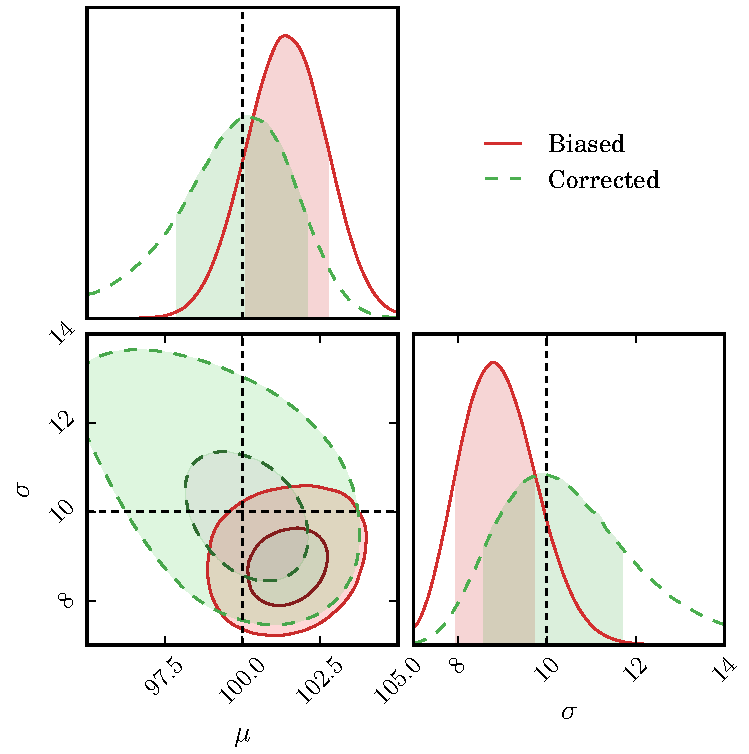
\includegraphics[width=\columnwidth]{example/imperfect.pdf}
	\end{center}
	\caption{A systematic test of our imperfect model, done by stacking the output chains from fitting 100 independent realisations of our 100 data points, subject to our thresholding.}
	\label{fig:imperfect}
\end{figure}

\section{The Real World}

Unfortunately it is a rare scenario when dealing with nature and all her faults for us to have an analytic selection function. Let alone a function encapsulated by a single parameter. A more realistic scenario involves a selection efficiency which cannot be conveniently described by an analytic function. Instead, we would have a high dimensional non-analytic function. And its probably stochastic too, just to throw another wrench in the works.


\section{Conclusion}
\label{sec:conclusion}



Still da bes


\section*{Acknowledgments}

We gratefully acknowledge the input of the many researchers that were consulted during the creation of this paper.


\bibliography{bibliography}


% Don't change these lines
\bsp	% typesetting comment
\label{lastpage}
\end{document}

% End of mnras_template.tex

